\chapter{Imperative Paradigm}
\label{ch:p1}

\section{Problem Statement}
\label{sec:pm1}

Compute distance between two documents.

\section{Data Structures and algorithms}

Some basic data structures like lists and dictionaries were used. Term frequency–inverse document frequency (Tf-Idf), is a numerical statistic that is intended to reflect how important a word is to a document in a collection or corpus. This method has been used to give weightage to more important words rather than just the word frequency.


\section{Methodology}

The entire methodology is divide into 4 stages. These include formatting text, creating word frequency vector, computing tf-idf weights and calculation of distance. 

\begin{figure}[H]
	\centering
	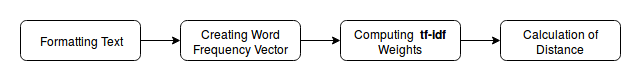
\includegraphics[height=0.12\textwidth,keepaspectratio]{flow_chart.png}\\
	\caption{The flow chart depicting stages of algorithm}
\end{figure}

\begin{itemize}
	\item \textbf{Formatting text :} Read the file and extract words from it. Words are obtained by splitting the text by various delimiters (variable \verb|delimiters|).
	\item \textbf{Word frequency vector :} After extracting the words, create a vector that contains the frequency of each and every word. This is done for each and every file in the corpus.
	\item \textbf{Computing tf-idf weights :} Tf-Idf weights corresponding to the above word frequency vector is calculated as per the given formula.
	\begin{center}
		$TF(t) = \frac{\text{Number of times term t appears in a document}}{\text{Total number of terms in the document}}$\\ 
		\vspace{1.2em}
		$IDF(t) = \ln \big( {\frac{\text{Total number of documents}}{\text{ Number of documents with term t in it}}} \big) $\\
		\vspace{1.2em}
		Tf-idf weight(t) = TF(t) * IDF(t)
	\end{center}
	\item \textbf{Calculation of distance :} The distance between each and every pair of files is done by calculating the cosine distance and later sorted. 
\end{itemize}

\section{Observations and results}
\label{sec:p01}

Some interesting observations have been found. Distance between same files is zero. 



\section{Contribution of team member}
